
\documentclass{standalone} 

\usepackage{tikz}
\usepackage{xcolor}
\usetikzlibrary{shapes.geometric, arrows}

\tikzstyle{startstop} = [rectangle, rounded corners, minimum width=3cm, minimum height=1cm, text centered, draw=black, fill=red!30]
\tikzstyle{io} = [trapezium, trapezium left angle=70, trapezium right angle=110, minimum height=1cm, text centered, draw=black, fill=blue!30]
\tikzstyle{process} = [rectangle, minimum width=1cm, minimum height=1cm, text centered, draw=black, fill=orange!30]
\tikzstyle{decision} = [diamond, minimum width=3cm, minimum height=1cm, text centered, draw=black, fill=green!30]
\tikzstyle{arrow} = [thick, ->, >=stealth]
\begin{document}
\nopagecolor 
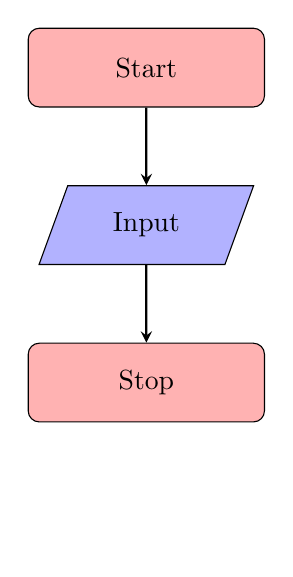
\begin{tikzpicture}[node distance=2cm]
\node(start)[startstop] {Start}; 
\node(in1)[io, below of=start]{Input};
\node(stop)[startstop, below of =in1] {Stop}; 
\node(footnote)[below of= stop] {}; 

\draw[arrow] (start) -- (in1); 
\draw[arrow] (in1) -- (stop);
\end{tikzpicture}
\end{document}
